\startchapter{Statistical Framework}
\label{chapter:stat}

This chapter presents the statistical framework used to search for evidence of new physics in the ATLAS collision data and, if no such evidence is found, establish the range of parameters over which the DH model is excluded by the search. Evidence of new physics would take the form of a statistically significant discrepancy between distributions of the observed collision data in the SRs compared with distributions of the predicted yield of SM background processes.

Owing to the observation of \ms-dependent peaks in the \minms distribution of the DH signal model in the SRs\footnote{See Section \ref{sec:minms} for details.}, the sensitivity of the search was found to be dramatically boosted by binning all data - MC simulated and ATLAS collision events - in the SRs into several bins of \minms prior to performing the statistical analysis. Details of the binning strategy are presented in Section \ref{sec:binning_strategy}. Within each analysis region and bin, the statistical analysis is performed by fitting the predicted yields of background and signal processes to the ATLAS collision data with the aim of maximizing the likelihood function presented in the following section. 

The computational construction and analysis of the likelihood function is performed within the HistFitter \cite{Baak_2015} statistical analysis framework.

\section{Likelihood Function}
\label{sec:likelihood}

The likelihood function which lies at the heart of the statistical framework is a product of Poisson distributions of event counts in all regions and bins:

\begin{equation}
\label{eq:likelihood_func}
\begin{aligned}
L(\boldsymbol{n}, \boldsymbol{\theta}^0|\mu_\text{Sig}, \boldsymbol{s}, \boldsymbol{\mu}, \boldsymbol{b}, \boldsymbol{\theta}) & = P_\text{SR} \times P_\text{CRs} \times C_\text{syst} \\
& = \prod_{i\in\text{SR bins}} P(n_{S,i}|\lambda_{S,i}(\mu_\text{Sig}, \boldsymbol{\mu_i}, s_i, \boldsymbol{b_i}, \boldsymbol{\theta})) \times \\ 
&\phantom{xxx}\prod_{j \in \text{CRs}} P(n_j|\lambda_j(\mu_\text{Sig}, \boldsymbol{\mu_j}, s_j, \boldsymbol{b_j}, \boldsymbol{\theta})) \times \\
&\phantom{xxx}C_\text{syst}(\boldsymbol{\theta}^0, \boldsymbol{\theta})
\end{aligned}
\end{equation}

where:

\begin{itemize}
    \item \(\boldsymbol{n}\in{n_{S,i}, n_j}\) is the set of all observed event counts in each region and bin.
    \item \(n_{S,i}\) and \(n_j\) are the number of observed events in the \(i^\text{th}\) bin of the SR and in the \(j^\text{th}\) CR, respectively.
    \item The signal strength \(\mu_\text{Sig}\) is an overall factor which scales the predicted yield of collision events produced by the DH signal model in all regions and bins.
    \item \(\boldsymbol{\mu}_{i(j)}\) represents the normalization factors in each bin \(i\) or region \(j\), which scale the \wjets and \ttbar backgrounds in all regions and bins of the fit. Separate normalization factors are used in the merged and resolved categories. The normalization factors are treated as unconstrained nuisance parameters (NPs) in the fit. They are initialized as 1, with an uncertainty of \(\pm1\).  
    \item \(s_{i(j)}\) is the yield of the signal process in each bin \(i\) or region \(j\) predicted by MC simulation. Likewise, \(\boldsymbol{b}_{i(j)}\) is the set of yield predictions for all SM background processes  in each bin \(i\) or region \(j\).
    \item \(\boldsymbol{\theta}\) represents the set of NPs that parametrize all uncertainties associated with the MC simulated yields. For each uncertainty source \(k\), the corresponding NP \(\theta_k\) continuously interpolates between the nominal value of the predicted yield and the up/down shifts associated with varying the given uncertainty source by \(\pm1\sigma\), as discussed in \Sect{4.4} of \Refn{~\cite{Baak_2015}}. For systematic sources, the NPs are normalized in the HistFitter framework such that \(\theta_k=0\) for the nominal yield and \(\theta_k=\pm1\) corresponds to \(\pm1\sigma\) variations of the uncertainty source. NPs associated with statistical uncertainty of the predicted yields are instead normalized such that \(\theta=1\) represents the nominal yield in the given bin and \(\theta_k=1\pm1\sigma_\text{stat}/N\) represents \(\pm1\sigma\) yield shifts, where N and \(\sigma_\text{stat}\) are the expected yield in the bin and its statistical uncertainty, respectively. 
    \item \(C_\text{syst}(\boldsymbol{\theta}^0, \boldsymbol{\theta})\) is a composite function of Gaussian priors which is used to constrain the floating NPs \(\boldsymbol{\theta}\) in the fit based on their central values \(\boldsymbol{\theta^0}\) and uncertainties \(\boldsymbol{\kappa}\):

    \begin{equation}
    \label{eq:gaussian_np}
    C_\text{syst}(\boldsymbol{\theta}^0, \boldsymbol{\theta})= \prod_{k\in S} \frac{1}{\kappa_k\sqrt{2\pi}}e^{-\frac{1}{2}(\frac{\theta^0_k-\theta_k}{\kappa})^2}
    \end{equation}
    \noindent where \(S\) is the full set of uncertainties considered in the fit.
    
    \item The Poisson expectation functions \(\lambda_{S,i}(\mu_\text{Sig}, \boldsymbol{\mu_i}, s_i, \boldsymbol{b_i}, \boldsymbol{\theta})\) and \(\lambda_j(\mu_\text{Sig}, \boldsymbol{\mu_j}, s_j, \boldsymbol{b_j}, \boldsymbol{\theta})\), represent the total expected yield in each SR bin \(i\) and CR bin \(j\), respectively. The Poisson expectation function is discussed in further detail in the following section.
\end{itemize}

\subsection{Poisson Expectation Function}
\label{sec:poisson_exp}

Within a given SR bin or CR \(k\), the Poisson expectation function \(\lambda_k\) in Eq. \ref{eq:likelihood_func} is given by:
    
\begin{equation}
\label{eq:lambda}
        \lambda_k(\mu_\text{Sig}, \boldsymbol{\mu_k}, s_k, \boldsymbol{b}_k, \boldsymbol{\theta}) = \mu_\text{Sig}s_k\eta_{k, \text{Sig}}(\boldsymbol{\theta}) + \sum\limits_{p\in{\text{\{SM bkg processes\}}}} \mu_{k,p} b_{k,p}\eta_{k,p}(\boldsymbol{\theta})
\end{equation}
    
\noindent where \(s_k\) (\(b_{k,p}\)) is the yield of the signal process (SM background process \(p\)) predicted by MC simulation, as discussed in Section \ref{sec:MC_ATLAS}. \(\eta_{i,s}(\boldsymbol{\theta})\) is a scaling factor, nominally set to 1, which parametrizes the variations in expected yield induced by varying the NPs \(\boldsymbol{\theta}\) in the fit:

        \begin{equation}
            \label{eq:sigma}
            \eta_{k,p}(\boldsymbol{\theta}) = 1 + \sum_{s\in\text{all systematics}}I(\theta_s(k,p), N_\text{down}(k,p), N_\text{up}(k,p))
        \end{equation}

        where \(I(\theta_p, \sigma_\text{down}(i,s), \sigma_{up}(i,s))\) is a continuous function of \(\theta_s(k,p)\) which interpolates\footnote{HistFitter employs a 6th-order polynomial to interpolate between  \(\sigma_\text{down}(i,s)\) and \(\sigma_\text{up}(k,p)\) a linear extrapolation beyond these extrema. See \Sect{4.1} of \Refn{~\cite{Cranmer:1456844}} for details.} the relative shift in predicted yields between the up \(N_\text{up}(k, p)\) and down \(N_\text{down}(k, p)\) extrema, associated with varying the given uncertainty source by \(\pm1\sigma\). 

\subsection{Nuisance Parameter Nomenclature and Correlations}
\label{sec:np_naming_corr}

Many of the NPs which appear in the likelihood function are correlated between bins, categories, and/or processes. For example, if a given NP is correlated between all bins in the fit, the value of the NP will be the same within all bins: \(\theta_s(k, p) \rightarrow \theta_s(p)\). The names given to NPs in the HistFitter framework reflect the presence of any such correlations by omitting the correlated information in the NP name. Taking the above example of an NP which is correlated between all bins, this correlation will be reflected by the omission of any bin number specification (eg. \verb|_bin1|).

The background normalization factors \(\boldsymbol{\mu}\) and uncertainty-related NPs \(\boldsymbol{\theta}\) are broken down as follows:

\begin{equation}
\label{eq:norm_factor_breakdown}
\boldsymbol{\mu}\in\{\mu_\text{\wjets, merged}, \mu_\text{\wjets, resolved}, \mu_\text{\ttbar, merged}, \mu_\text{\ttbar, resolved}\}
\end{equation}

\noindent and

\begin{equation}
\label{eq:norm_factor_breakdown}
\boldsymbol{\theta}\in\{\boldsymbol{\theta}_\text{statistical}, \boldsymbol{\theta}_\text{sys, experimental}, \boldsymbol{\theta}_\text{sys, theory}\}
\end{equation}

Table \ref{tab:np_naming} summarizes the correlations present for each type of NP, and the scheme used by HistFitter to assign names to each.

\begin{table}
\centering
\caption{Summary of naming scheme and correlation information for nuisance parameters in the likelihood function. See Tables \ref{tab:exp_syst_naming} and \ref{tab:theo_syst_naming} for details of the names assigned to NPs associated with individual sources of systematic uncertainty.}
\label{tab:np_naming}
\footnotesize{
\begin{tabular}{p{2.5cm} p{4cm} p{4cm} p{3.5cm} }
\toprule
\textbf{NP Type} & \textbf{Description} & \textbf{Correlation Info} & \textbf{Naming Scheme} \\
\midrule
\midrule
\(-\) \(\mu_\text{\wjets, mgd}\) \newline \(-\) \(\mu_\text{\wjets, res}\) \newline \(-\) \(\mu_\text{\ttbar, mgd}\) \newline \(-\) \(\mu_\text{\ttbar, res}\) & Normalization factor which scales the \wjets (\ttbar) background in all analysis regions and bins of the merged (resolved) category. & Correlated between all analysis regions and bins for the \wjets (\ttbar) background in the merged (resolved) category. Each normalization factor scales one process (\ttbar or \wjets) - i.e. no correlation between processes. & \(-\) \(\mu\){\uscore}Wjets{\uscore}mgd \newline \(-\) \(\mu\){\uscore}Wjets{\uscore}res \newline \(-\) \(\mu\){\uscore}ttbar{\uscore}mgd \newline \(-\) \(\mu\){\uscore}ttbar{\uscore}res \\
\midrule
\(\boldsymbol{\theta}_\text{statistical}\) & NPs which parametrize the statistical uncertainty associated with the predicted yield in each region and bin from MC simulation. & Correlated between all processes. Not correlated between regions or bins.  & \(\gamma\){\uscore}\{region\}{\uscore}\{category\}{\uscore}\newline\{bin type\}{\uscore}bin{\uscore}\newline\{bin index\} \\
& & \begin{equation}\nonumber \phantom{xxxxxxxxxxxxx} \text{bin type}=\begin{cases} \text{``mS{\uscore}bin"} & \text{in SR bins} \\ \text{``cuts"} & \text{in CRs} \end{cases}\end{equation}   \\
\midrule
\(\boldsymbol{\theta}_\text{sys, experimental}\) & NPs which parametrize systematic uncertainties from experimental sources. & Correlated between all processes, regions and bins.  & \(\alpha\){\uscore}\{uncertainty source\} \\
\midrule
\(\boldsymbol{\theta}_\text{sys, theory}\) & NPs which parametrize systematic uncertainties for each process from theoretical sources. & Correlated between all regions and bins. Not correlated between processes.  & \(\alpha\){\uscore}{process}{\uscore}\newline\{uncertainty source\} \\
\bottomrule
\end{tabular}}
\end{table}

Table \ref{tab:exp_syst_naming} (\ref{tab:theo_syst_naming}) summarizes the scheme used to name NPs associated with the experimental (theoretical) uncertainty sources presented in Chapter \ref{chapter:systematics}.

\section{Binning Strategy}
\label{sec:binning_strategy}

As shown in Figure \ref{fig:minms_shape_discrimination}, the \minms variable presented in Section \ref{sec:minms} has a \ms-dependent peaked distribution which for most \ms values is distinct in shape from the distribution of SM background processes in this variable. This shape discrimination between the signal and background processes is exploited when performing the likelihood fit by binning the MC simulated events and collision data into several \minms bins. 

\begin{figure}[htbp]
  \centering
    \begin{subfigure}[t]{0.48\textwidth}
    \centering
     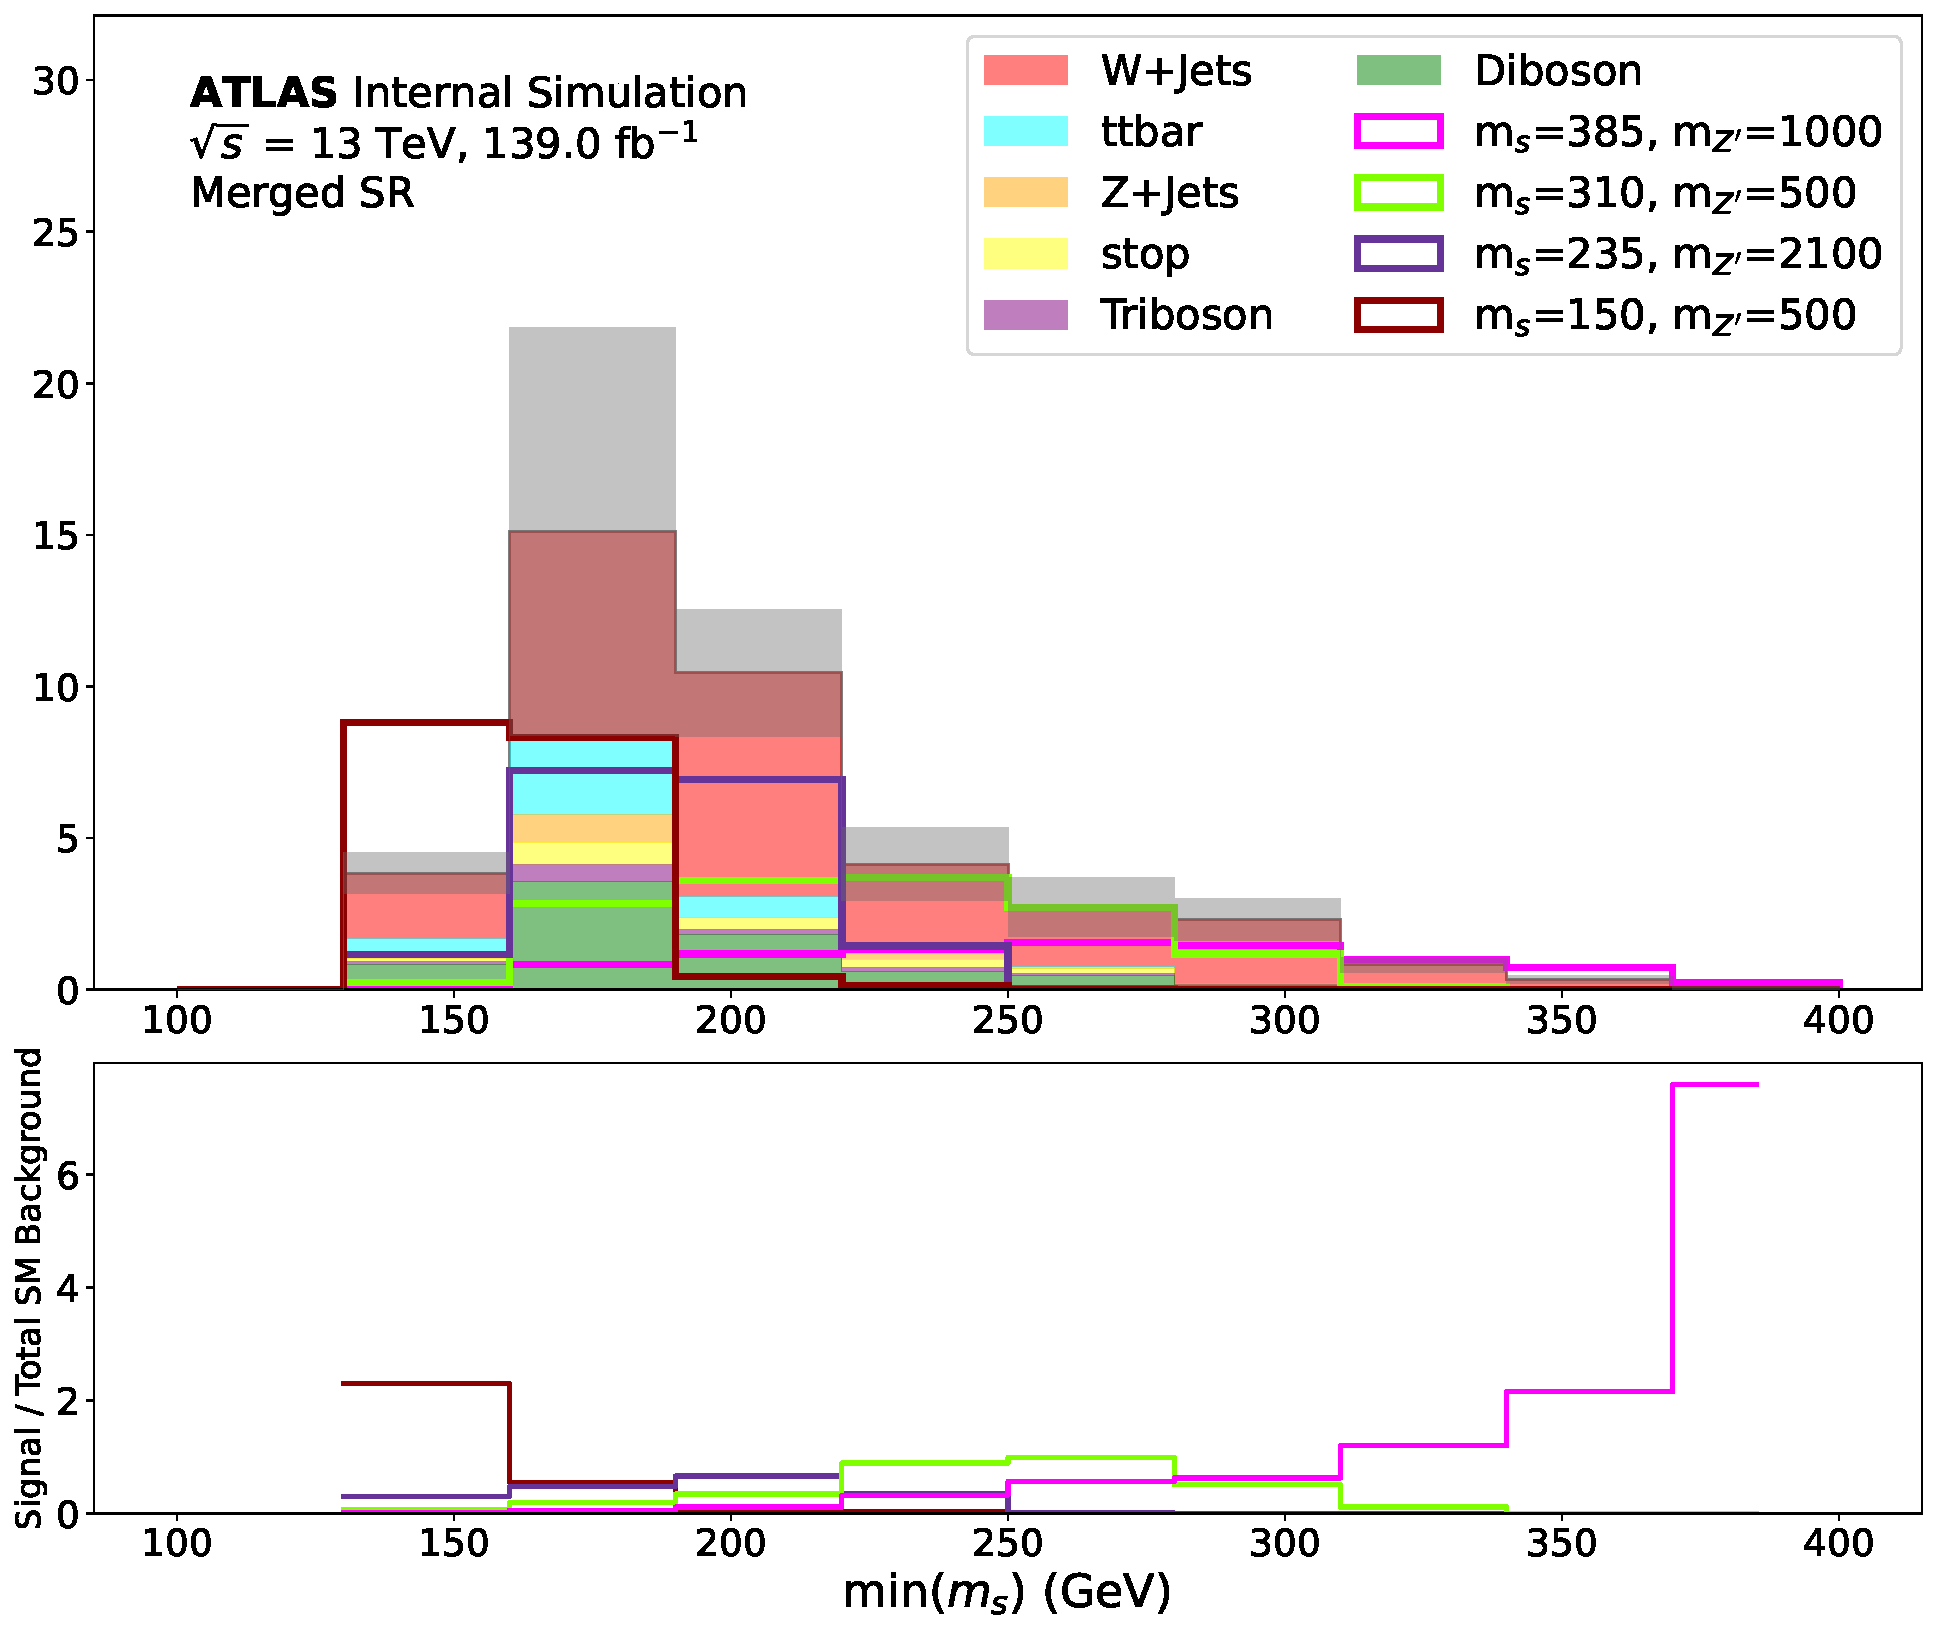
\includegraphics[width = 0.99\textwidth]{Figures/7/SR1L_Merged/TARJets10_minmS_mgd.pdf}
    \caption{Merged SR}
    \end{subfigure}
    \begin{subfigure}[t]{0.48\textwidth}
    \centering
     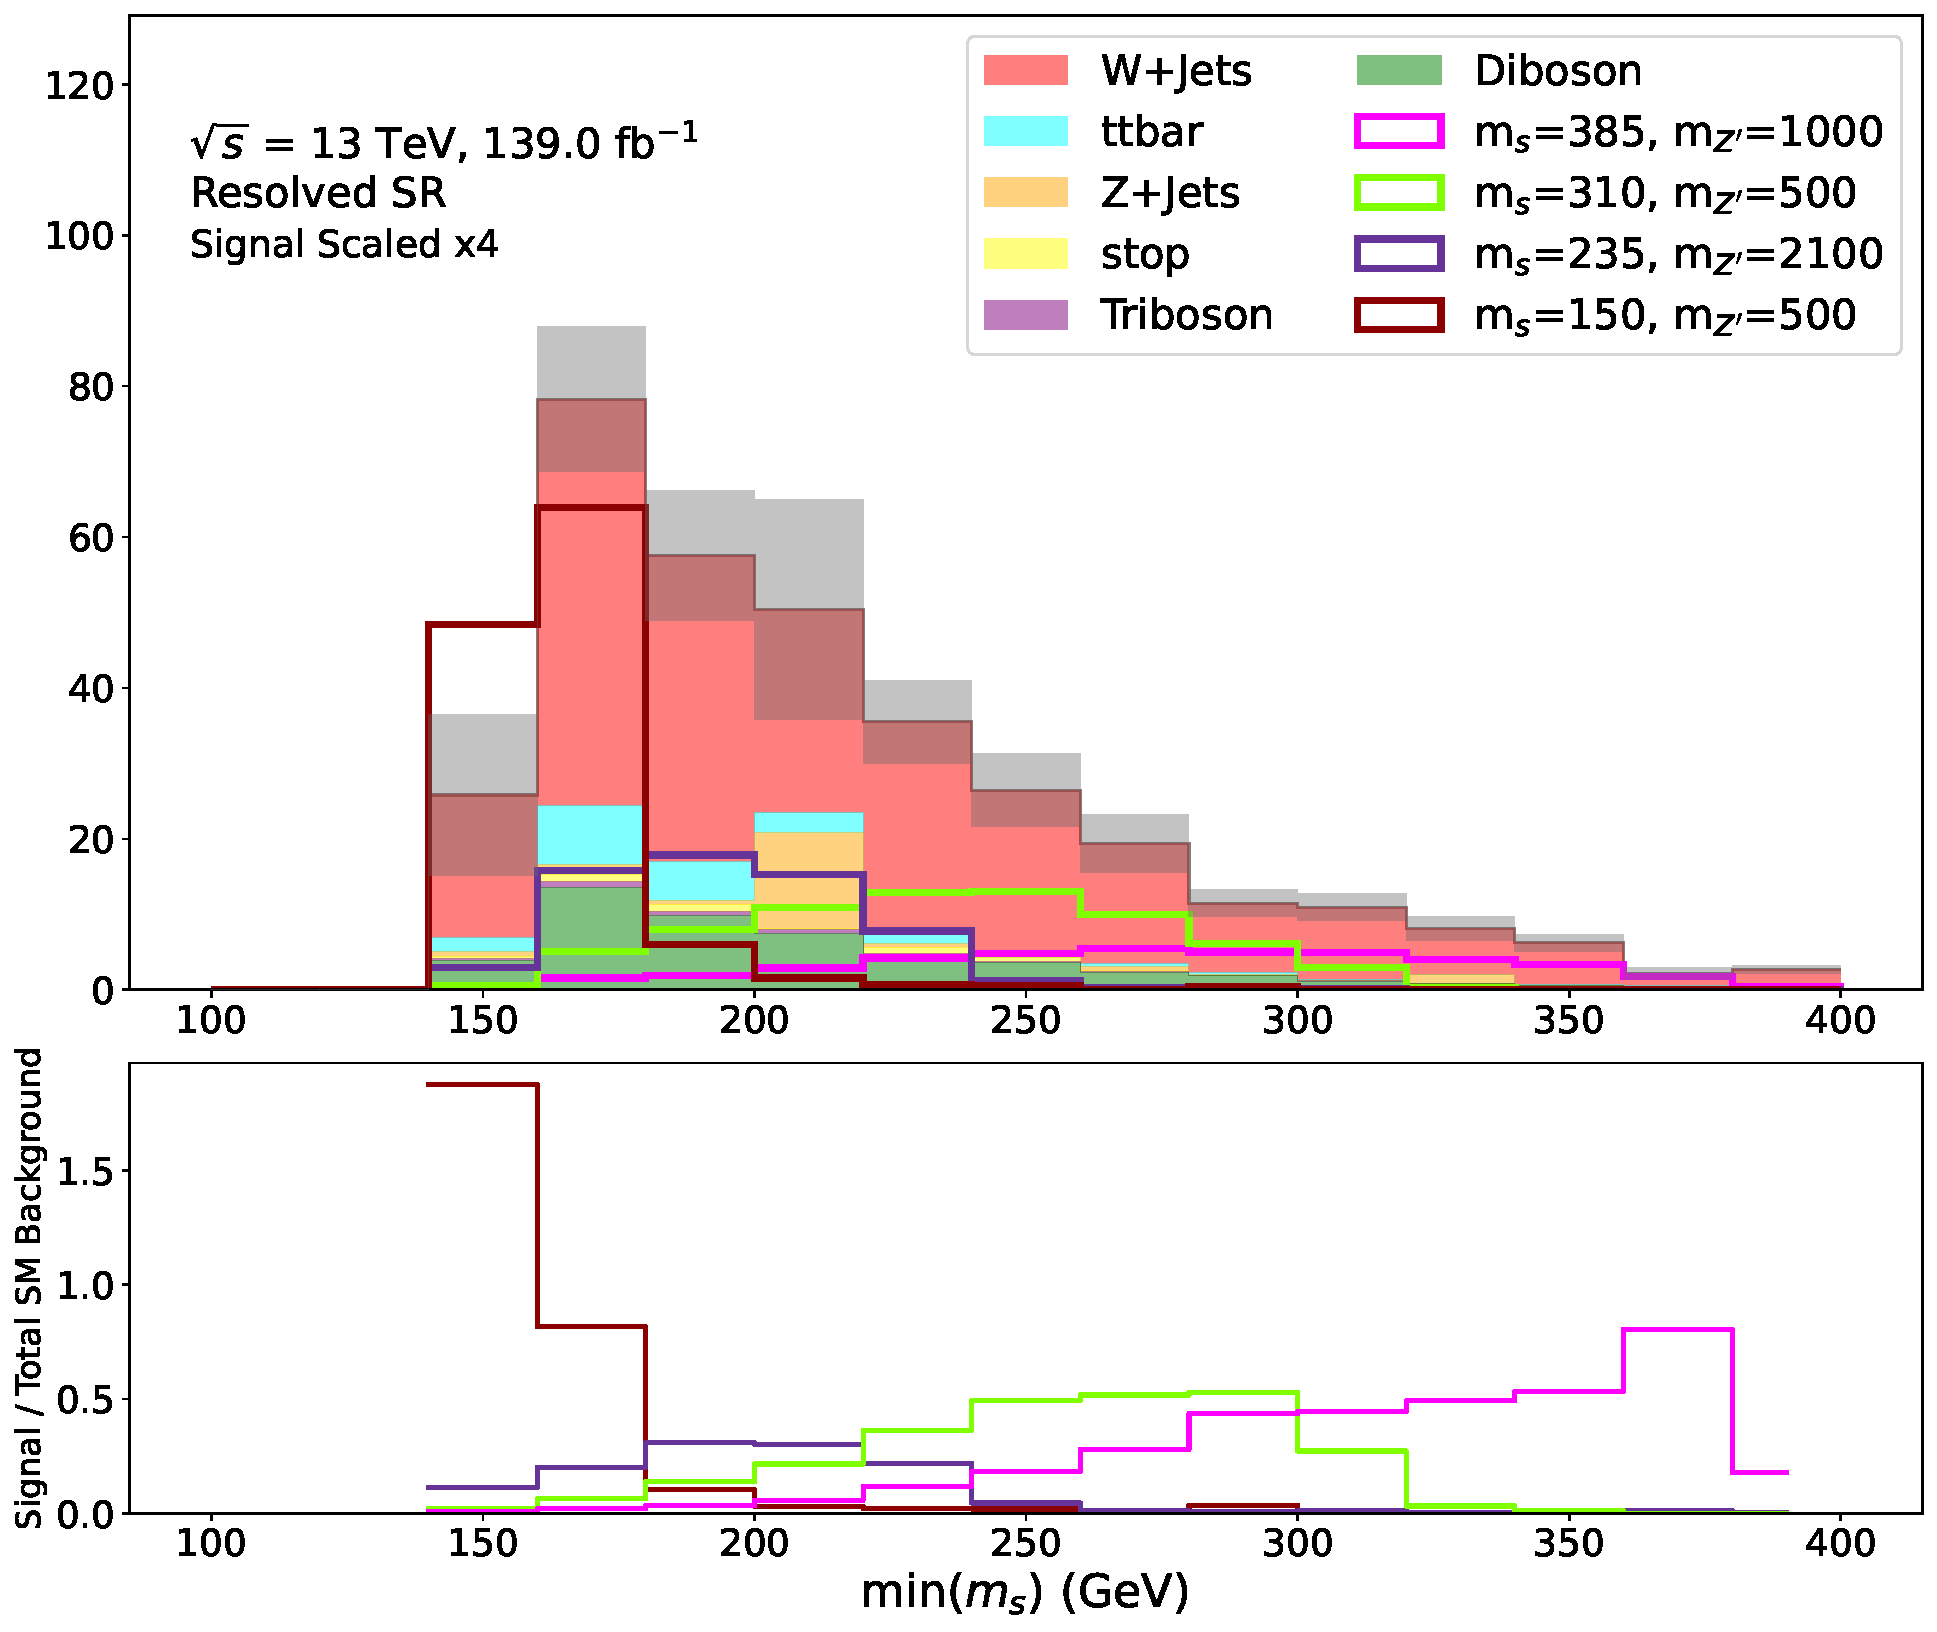
\includegraphics[width = 0.99\textwidth]{Figures/7/SR1L_Resolved/TARJets10_minmS_res.pdf}
     \caption{Resolved SR}
    \end{subfigure}
    \caption{Predicted yields of SM background processes (stacked filled) and the DH signal model (unfilled lines) at several mass points in the merged (left) and resolved (right) SRs, binned in \minms. The lower panel shows the ratio of yields predicted for the DH signal process over the sum of MC background processes. Grey bands show the statistical uncertainty of the background estimate.}
   \label{fig:minms_shape_discrimination}
\end{figure}


The exact placement of bin edges in \minms used when performing the fit was optimized with the aim of maximizing the projected exclusion of the DH signal model for a background-only hypothesis using the limit-setting strategy presented in Section \ref{sec:hypo_test}, while maintaining a total predicted yield of \(>5\) SM background events in each bin to justify the use of the asymptotic approximation during limit-setting (see Section \ref{sec:hypo_test} for details). 

Distributions of \minms are shown with the optimized binning in Figure \ref{fig:minms_binning}. In the merged SR, binning the data into four \minms bins with non-equidistant bin edges was found to provide maximal sensitivity while maintaining \(>5\) predicted SM background events per bin. In the resolved SR, binning into five \minms bins was found to be optimal, and equidistant bin edges are used because no appreciable sensitivity improvements were found with non-equidistant edges.

\begin{figure}[htbp]
  \centering
    \begin{subfigure}[t]{0.48\textwidth}
    \centering
     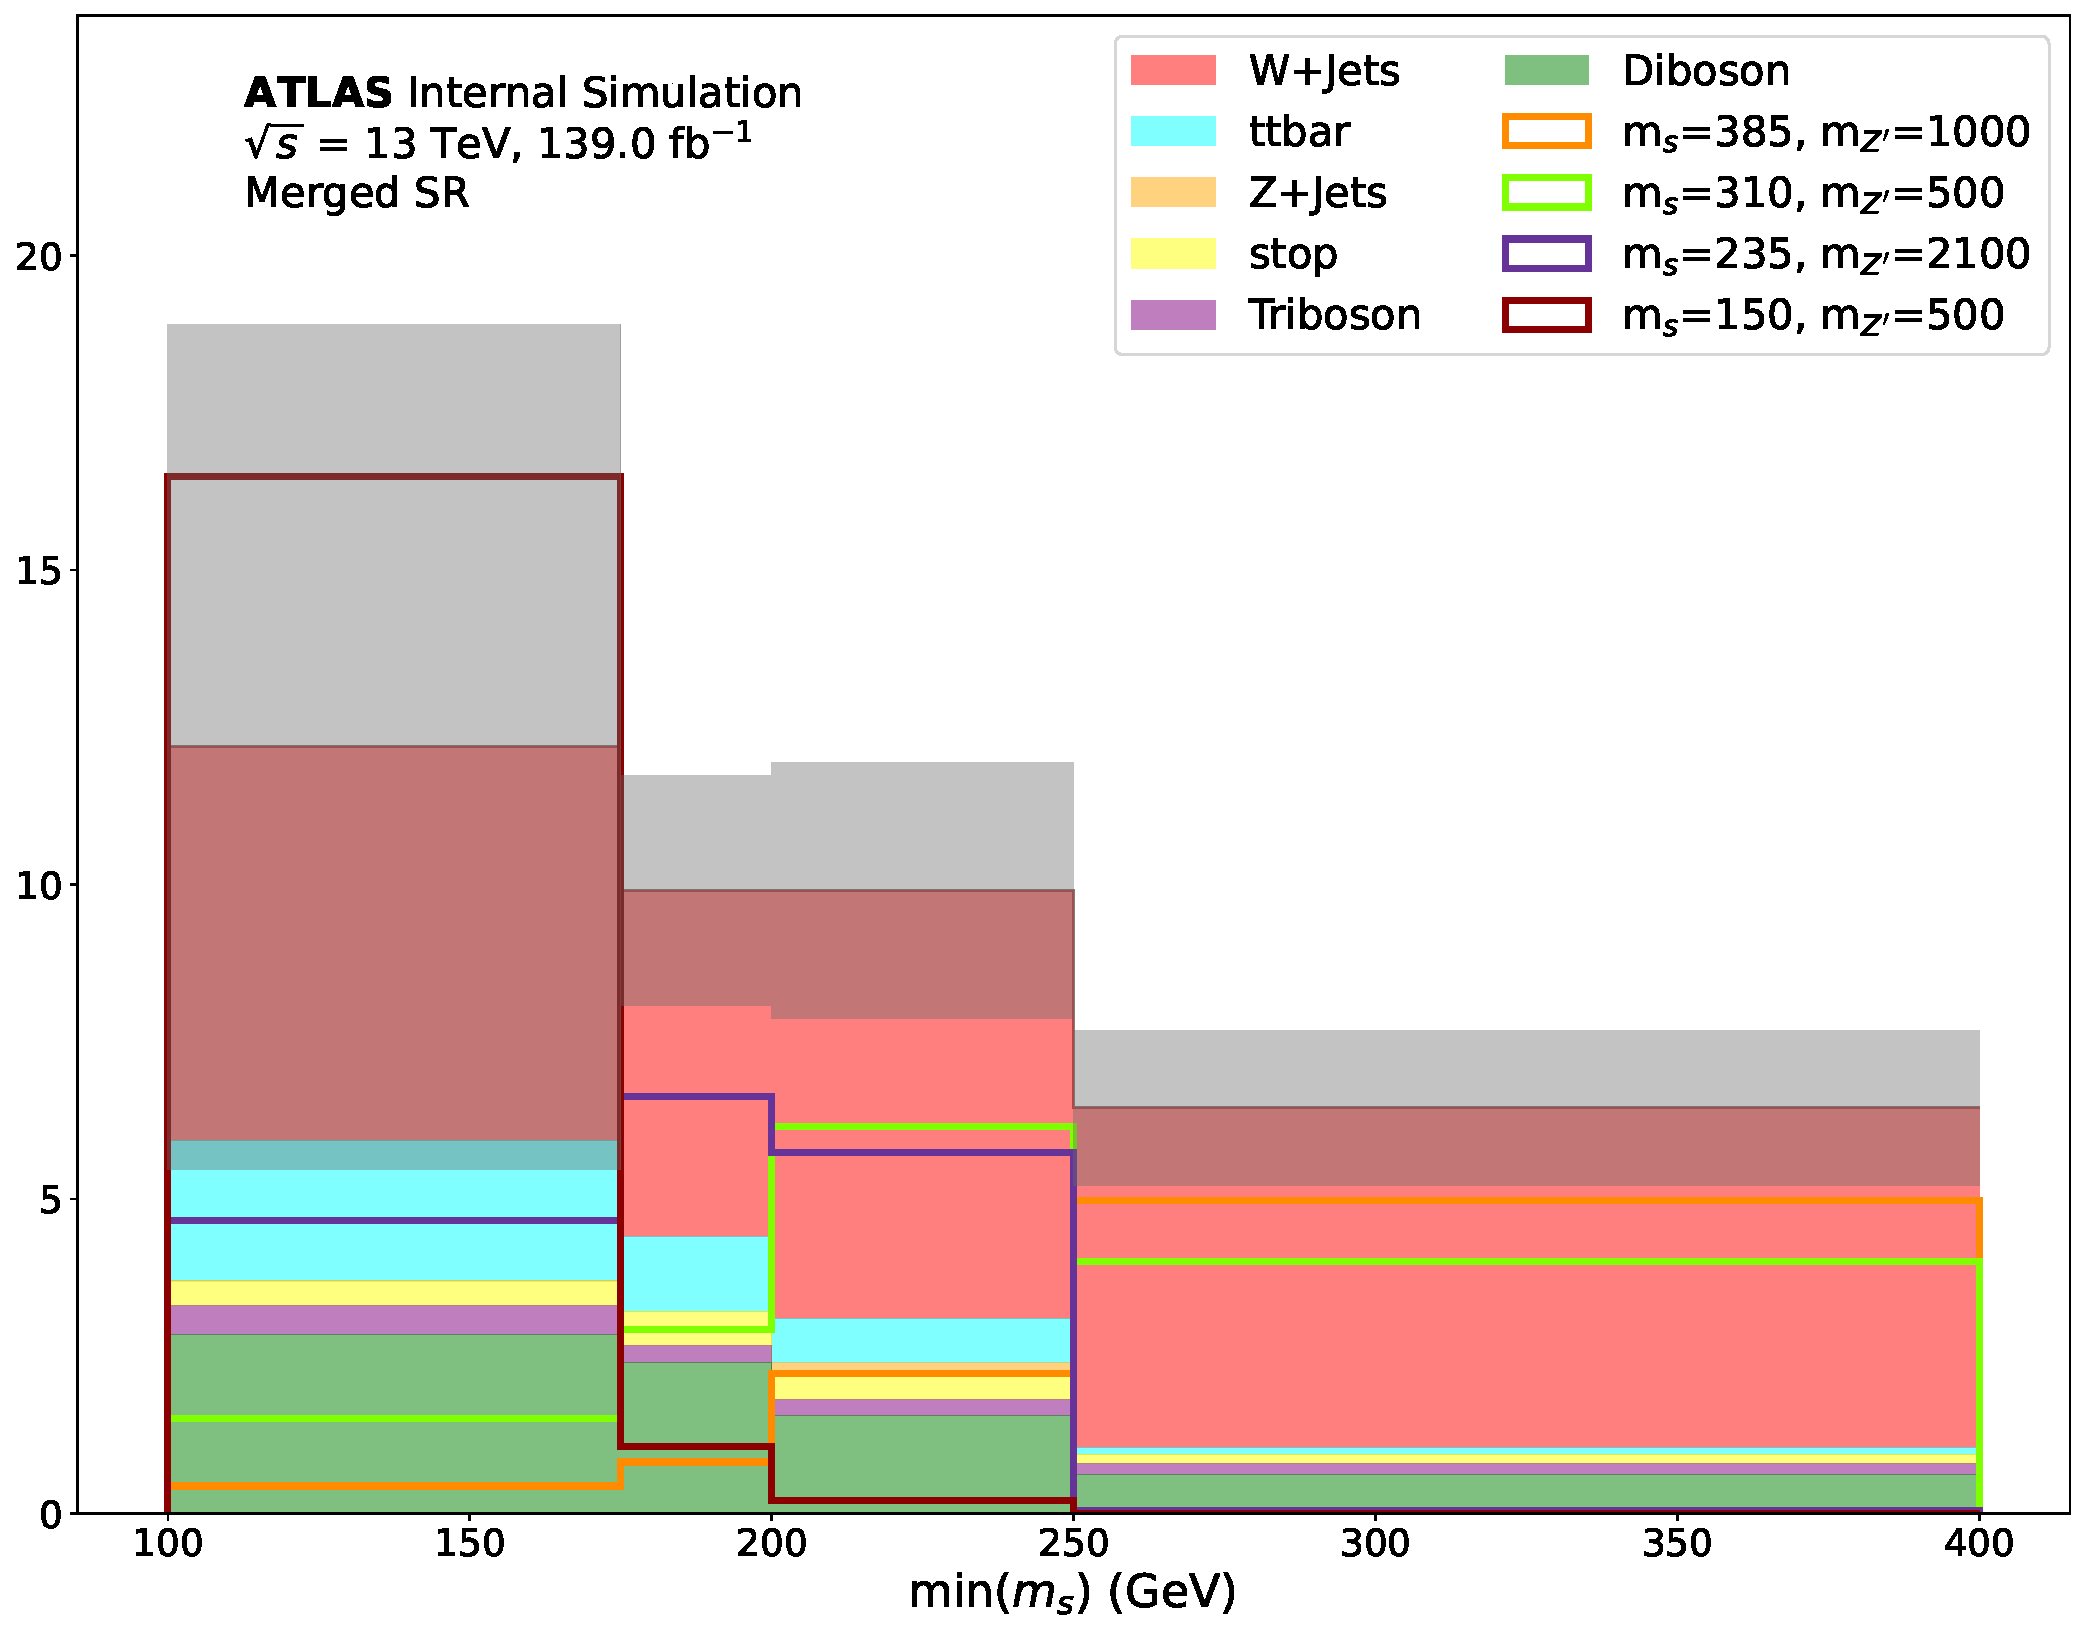
\includegraphics[width = 0.99\textwidth]{Figures/7/SR1L_Merged_fit/TARJets10_minmS_mgd.pdf}
    \caption{Merged SR}
    \end{subfigure}
    \begin{subfigure}[t]{0.48\textwidth}
    \centering
     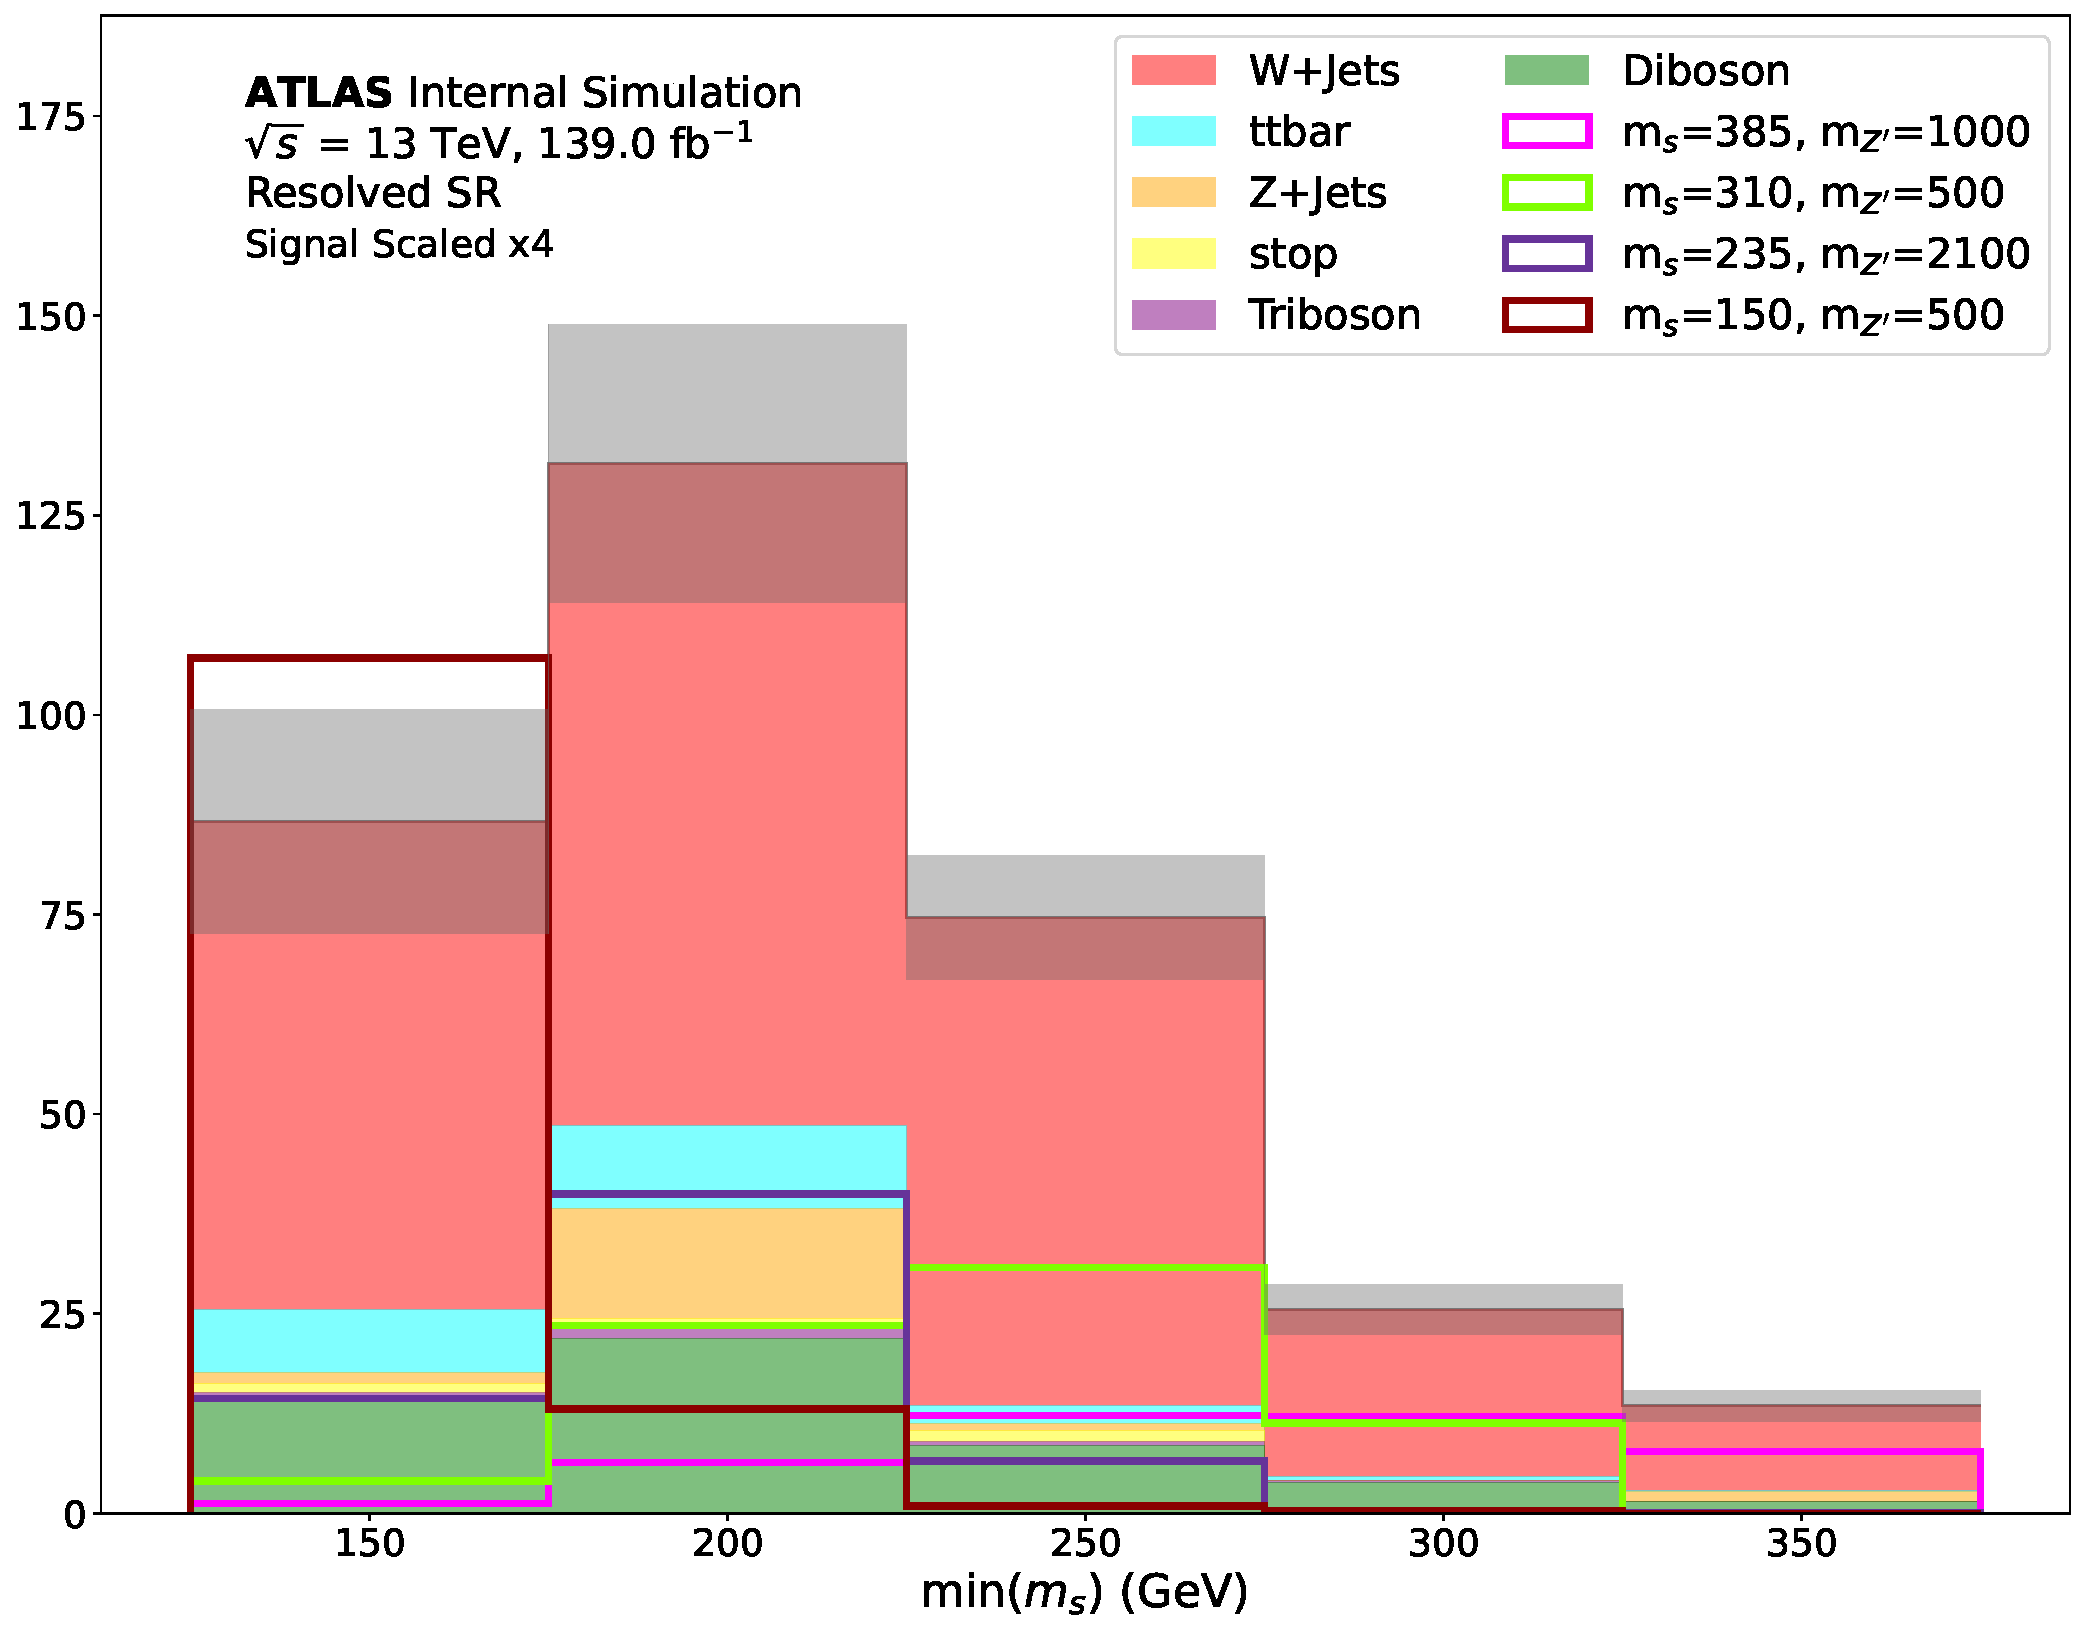
\includegraphics[width = 0.99\textwidth]{Figures/7/SR1L_Resolved_fit/TARJets10_minmS_res.pdf}
     \caption{Resolved SR}
    \end{subfigure}
    \caption{Predicted yield of SM background processes (stacked filled) and the DH signal model (unfilled lines) at several mass points in the merged (left) and resolved (right) SRs, binned in \minms with the optimized bin edges presented in Table \ref{tab:statisticalevaluation_regions}. Grey bands show the statistical uncertainty of the background estimate.}
   \label{fig:minms_binning}
\end{figure}

The CRs are left unbinned in the fit to provide constraints on the overall yield of the \wjets and \ttbar processes in each kinematic category. Table \ref{tab:statisticalevaluation_regions} summarizes the binning strategy in all analysis regions.

\begin{table}[ht]
\centering
\footnotesize{
    \caption{Binning used in the regions entering the statistical analysis.}
    \label{tab:statisticalevaluation_regions}
    \begin{tabular}{l ll}
    \toprule
    \textbf{Region}         &  \textbf{Binning in Merged Category} & \textbf{Binning in Resolved Category} \\
    \midrule
    \midrule
    \multirow{2}{*}{SR} & 4 non-equidistant bins in \(m_s\) & 5 equidistant bins in \(m_{s}\)  \\
    					     & bin edges: [125, 165, 190, 225, 375] \GeV & bin edges: [125, 175, 225, 275, 325, 375] \GeV \\
    \midrule   					   
    \wjets CR & none & none \\
    \midrule    
    \ttbar CR & none  & none \\ 
    \bottomrule
    \end{tabular}}
\end{table}

\section{Fit Setup}
\label{sec:fit_setup}

With the MC simulated yields and ATLAS collision data binned into CRs and \minms bins within the SRs, as detailed in Section \ref{sec:binning_strategy} above, the statistical analysis is performed by fitting the simulated yields to the collision data in all regions and bins. The fits are performed within the HistFitter framework by varying the signal strength parameter \(\mu_\text{Sig}\) and all floating NPs \(\{\boldsymbol{\mu}, \boldsymbol{\theta}\}\) in the likelihood function presented in Eq. \ref{eq:likelihood_func}, until the set of parameter values which maximizes the likelihood is determined.  

\subsection{Pruning of Systematics}
\label{sec:pruning}

Prior to performing a fit, NPs associated with systematic uncertainties are pruned within the HistFitter framework at a user-defined threshold. The pruning is done as follows: for a given source of systematic uncertainty, HistFitter compares the relative up and down yield shifts due to a given NP within each analysis region and bin. If the relative shift in both directions is below the user-defined threshold in all regions and bins, the given NP is `pruned', which means that it is not included in fit. Pruning helps to reduce fitting time, as well as minimizing numerical instabilities in the fit. 

For this search, a 1\% pruning threshold is applied. Dedicated studies were done to ensure that the impact of pruning systematics at a 1\% threshold has no appreciable impact on the overall fit behaviour or search results. 

\subsection{Background-only Fit and Signal Region Extrapolation}
\label{sec:extrapolation}

To initially check for an excess of data in the SRs, a ``background-only" fit of the SM background yield prediction to the observed collision data is performed in the CRs to constrain the normalization factors (eg. \(\mu_\text{\wjets, mgd}\)) for the \wjets and \ttbar backgrounds within each category, along with all other NPs \(\boldsymbol{\theta}\) that affect yields expectations in the CRs. The likelihood function presented in Eq. \ref{eq:likelihood_func} is modified such that \(\mu_\text{Sig}\) is fixed to 0 (i.e. ``background-only"), and the SR component \(P_\text{SR}\) is fixed to 1 (i.e. ``CR-only"). 

The values of normalization factors and other NPs which are constrained in the background-only fit to maximize this modified likelihood function are subsequently extrapolated to SR to incorporate these constraints into the predicted yields of background processes in the SR. The updated distributions of the total  predicted SM background yield in the SR are compared with distributions of the observed collision data to check for the presence of any  discrepancies which, if statistically significant considering all statistical and systematic uncertainties, would be indicative of new physics in the data. 

The extrapolation to the SR is performed by building the total expected yield of SM background events in each SR bin using the Poisson expectation formula in Eq. \ref{eq:lambda} with the constrained NPs, and with \(\mu_\text{Sig}\) still set to 0. Any NPs which are specific to the SR and thus not constrained in the background-only fit are maintained at their nominal pre-fit values when constructing the extrapolated Poisson expectations. Further details of the extrapolation method and its implementation within the HistFitter framework can be found in Section 5.2 of \Refn{~\cite{Baak_2015}}.

\subsubsection{Evaluation of Systematic Uncertainties by Means of the Transfer Factor}
\label{sec:TF}
After the values of all background normalization factors \(\boldsymbol{\mu}\) are constrained in the background-only fit, the total yield \(\big((b_\text{fit})_{p,\text{ mgd CRW}} + 
(b_\text{fit})_{p,\text{ mgd CRTT}}\big)\) of a process \(p\) (either \wjets or \ttbar) in the merged CRs whose normalization factor \(\mu_{p\text{,mgd}}\) is constrained in the fit can be expressed using the formalism of Eq. \ref{eq:lambda} (neglecting for now the \(\boldsymbol{\theta}\) constraints) as:

\begin{small}
\begin{equation}
\label{eq:normfactor}
(b_\text{fit})_{p,\text{ mgd CRW}} + 
(b_\text{fit})_{p,\text{ mgd CRTT}} = 
\mu_{p\text{,mgd}} \Big[b_{p,\text{ mgd CRW}}  + 
b_{p,\text{ mgd CRTT}}\Big]
\end{equation}
\end{small}

\noindent where an equivalent formula would apply in the resolved CRs with ``mgd"\(\rightarrow\)``res".

%After extrapolating the normalization factors from the background-only fit to the SRs as described in Section \ref{sec:extrapolation} above, the extrapolated estimate of the

Extrapolating the constrained normalization factor \(\mu_{p\text{,mgd}}\) to any region or bin \(j\) in the merged category scales the predicted yield of the process \(p\) in a bin \(j\) of the merged SR as follows:

\begin{equation}
\label{eq:extrapolation}
\begin{aligned}
(b_\text{fit})_\text{\(p\), \(j\)} &= \mu_{p\text{,mgd}} \times b_\text{\(p\), \(j\)}  \\
&= \Big[(b_\text{fit})_{p,\text{ mgd CRW}} + (b_\text{fit})_{p,\text{ mgd CRTT}}\Big] \times 
\Bigg[\frac{b_\text{\(p\), \(j\)}}{b_{p,\text{ mgd CRW}}  + b_{p,\text{ mgd CRTT}}}\Bigg]
\end{aligned}
\end{equation}

The ratio of raw MC yields in brackets which extrapolates the fitted yield \(\big((b_\text{fit})_{p,\text{ mgd CRW}} + (b_\text{fit})_{p,\text{ mgd CRTT}}\big)\) of process \(p\) in the merged CRs to the estimated yield \((b_\text{fit})_\text{\(p\), \(j\)}\) in a given region or bin \(j\) is referred to as the ``transfer factor" \(TF\).

When considering how the systematic uncertainties, which are correlated between regions and bins, can be expected to impact the predicted yields \((b_\text{fit})_\text{\(p\), \(j\)}\), the fitted yield of the process \(p\in\{\wjets, \ttbar\}\) in the CRs will be predominantly set by the observed yield of collision data, and consequently should be effectively unshifted when systematic uncertainty sources are varied. As a result, the primary impact of systematic uncertainty sources on the predicted yields \((b_\text{fit})_\text{\(p\), SR bin \(j\)}\) in the SR will take the form of correlated shifts of the predicted yields on the top and bottom of the \(TF\) ratio. For this reason, relative systematic uncertainties associated with the post-fit predicted yields in all regions are evaluated for the \wjets and \ttbar backgrounds using systematic shifts in the \(TF\) rather than in the pre-fit yields. In a given SR bin or CR \(j\) in the merged category:

\begin{equation}
\label{eq:tf_unc}
\begin{aligned}
\text{rel. syst}\text{(TF, sys up, \(p\), \(j\) (mgd)} &= \frac{TF(\text{sys up, \(p\), \(j\) (mgd))}}{TF_\text{nom}} \\ 
&= \Bigg[\frac{b_\text{\(p\), sys up, \(j\) (mgd)}}{b_\text{\(p\), \(j\) (mgd)}}\Bigg] \times \\
& \phantom{xxl} \Bigg[\frac{b_{p,\text{ mgd CRW}}  + b_{p,\text{ mgd CRTT}}}{b_{p,\text{ sys up, mgd CRW}}  + b_{p,\text{ sys up, mgd CRTT}}}\Bigg] -1
\end{aligned}
\end{equation}

\noindent where an analogous equation holds in the resolved category with "mgd"\(\rightarrow\)"res". 

If yield shifts associated with a given systematic source are positively correlated between the region or bin \(j\) and the CRs and comparable in size relative to the nominal yield, then the relative systematic uncertainty of the transfer factor can be significantly reduced compared with that of the raw yields due to cancellation between the two terms in square brackets in Eq. \ref{eq:tf_unc}. 

Table \ref{tab:TF_sys_comp} compares the total relative systematic uncertainty associated with the predicted yield of the \wjets process in the SRs (bins combined) and \wjets CRs, evaluated using either the systematic yield uncertainties alone (first term in square brackets in Eq. \ref{eq:tf_unc}) or using the \(TF\). The \ttbar CRs are excluded from the comparison due to the relatively small predicted yield of \wjets events in these CRs. The combination of systematic uncertainties from all sources is performed within the HistFitter framework. The relative systematic uncertainties are reduced in all regions when evaluated using the \(TF\) rather than the yield. In the \wjets CR (CRW), much of the reduction comes from the fact that most of the \wjets events in the combined CRW+CRTT are contained within the CRW, so systematic shifts in the combined CRW+CRTT yield are guaranteed to be highly correlated with those in the CRW. 

\begin{table}[ht]
\begin{center}
\caption{\label{tab:TF_sys_comp} Comparison of total relative systematic uncertainty associated with the predicted yield of the \wjets process in the SRs and \wjets CRs (CRW), evaluated using either the predicted yield (second column) or the \(TF\) (third column). The relative statistical uncertainty is shown in the first column for comparison.}
\begin{tabular}{l l l l }
\toprule
\textbf{Analysis Region} &\textbf{Stat} &\textbf{Total Sys (yield)} & \textbf{Total Sys (TF)} \tabularnewline
\midrule
\midrule
Merged SR & \(\pm\)14\% & \(\pm\)31\% & \(\pm\)27\% \tabularnewline
\midrule
Resolved SR & \(\pm\)7\% & \(\pm\)24\% & \(\pm\)14\% \tabularnewline
\midrule
Merged CRW & \(\pm\)11\% & \(\pm\)24\% & \(\pm\)12\% \tabularnewline
\midrule
Resolved CRW & \(\pm\)4\% & \(\pm\)16\% & \(\pm\)4\% \tabularnewline
\bottomrule
\end{tabular}
\end{center}
\end{table}

\subsection{Exclusion Hypothesis Test and Limit Setting}
\label{sec:hypo_test}

In the event that no significant discrepancy is seen in the comparison of SM background yield predictions to the ATLAS collision data in the SR following the background-only fit and extrapolation of constraints to the SR, an exclusion hypothesis test of the DH signal model is performed at each simulated \ms and \mZp to assess the range, or ``limits", of model parameters that can be excluded by the search. This procedure is referred to as ``limit setting".

The exclusion hypothesis test is performed using ``signal+background fits", which incorporate all regions and bins in the likelihood function presented in Eq. \ref{sec:likelihood}, and allow for a nonzero signal strength \(\mu_\text{Sig}\). The ultimate product of the hypothesis test at each \ms and \mZp of the DH model is a ``CL\(_s\) value". A CL\(_s\) value below 0.05 is considered to exclude the signal+background hypothesis at a 95\% confidence level (CL).

Typical approaches to evaluating a CL associated with an alternative hypothesis directly consider the level of agreement between the observed data and the expectation of the alternative hypothesis. In the context of a search for new phenomena in experimental particle physics, this amounts to evaluating the confidence level CL\(_{s+b}\) associated with the signal+background hypothesis. The CL\(_{s+b}\) approach encounters issues when one considers a regime in which the data is expected to be predominantly comprised of background events (\(s<<b\)). In this regime, CL\(_{s+b}\) becomes increasingly similar to the confidence level CL\(_{b}\) associated with the null background-only hypothesis; this effect tends to diminish the ability of the search to exclude the signal+background hypothesis at a fixed reference CL (eg. 95\%). To address this issue, the CL\(_s\) method considers instead the CL\(_s\) ratio:

\begin{equation}
\label{eq:CLs_method}
\text{CL}_s = \frac{\text{CL}_{s+b}}{\text{CL}_{b}}
\end{equation}

\noindent which compares the confidence with which the observed data can be explained by the alternative signal+background hypothesis relative to the null background-only hypothesis. The CL\(_s\) is generally found to provide more powerful exclusion than the CL\(_{s+b}\) in the high-background regime.

\subsubsection{CL\(_s\) Evaluation Strategy}

For a given value of the hypothesized signal strength \(\mu_\text{Sig}\), a ``profiled log-likelihood ratio" \(q_{\mu_\text{Sig}}\) is constructed as follows:

\begin{equation}
\label{eq:prof_likelihood_ratio}
q_{\mu_\text{Sig}} = -2\log\Bigg( \frac{L(\mu_\text{Sig}, \boldsymbol{\hat{\hat{\theta}}})}{L(\hat{\mu}_\text{Sig}, \boldsymbol{\hat{\theta})}} \Bigg)
\end{equation}

\noindent where \(\hat{\mu}_\text{Sig}\) and \(\boldsymbol{\hat{\theta}}\) are the values of \(\mu_\text{Sig}\) and of the NPs \(\boldsymbol{\theta}\) that maximize the likelihood function with all parameters left floating (i.e. profiled over) in the signal+background fit. \(\boldsymbol{\hat{\hat{\theta}}}\) is the set of floating NP values that maximize the likelihood function for a given fixed \(\mu_\text{Sig}\) in the fit. Note that the background normalization parameters \(\boldsymbol{\mu}\) are folded into the set of NPs \(\boldsymbol{\theta}\) in Eq. 
\ref{eq:prof_likelihood_ratio}, and in all equations which follow in this section.

Two p-values are evaluated to quantify the CL\(_{s+b}\) (CL\(_b\)) by integrating the distribution \(f(q_{\mu_\text{Sig}}|\mu_\text{Sig}, \boldsymbol{\theta})\) above (below) the value \(q_{\mu_\text{Sig},\text{ obs}}\) evaluated for \(\mu_\text{Sig}=1\) (\(\mu_\text{Sig}=0\)) with the observed ATLAS collision data and the central NP values input to the fit:

\begin{equation}
\label{eq:pvalue_CLs_b}
\text{CL}_{s+b} = p_{\mu_\text{Sig}=1} = \int_{q_{1},\text{ obs}}^\infty f(q_{1}|\mu_\text{Sig}=1, \boldsymbol{\theta})dq_{1}
\end{equation}

\begin{equation}
\label{eq:pvalue_CLb}
\text{CL}_{b} = p_{\mu_\text{Sig}=0} = \int_{-\infty}^{q_0,\text{ obs}} f(q_{0}|\mu_\text{Sig}=0, \boldsymbol{\theta})dq_{0}
\end{equation}

The distribution \(f(q_{\mu_\text{Sig}}|\mu_\text{Sig}, \boldsymbol{\theta})\) can be obtained by throwing pseudo-experiments which randomize the number of observed events and the central values of the NPs \(\boldsymbol{\theta}\), and re-calculating \(q_{\mu_\text{Sig}}\) for each pseudo-experiment. However, for sufficiently high statistics in the analysis regions - typically taken to be at least \(\mathcal{O}(5)\) expected SM background events per region or bin - \(f(q_{\mu_\text{Sig}}|\mu_\text{Sig}, \boldsymbol{\theta})\) is known to follow a \(\chi^2\) distribution according to Wilks' theorem \cite{Wilks_1938}. In this ``asymptotic regime", asymptotic formulae \cite{Cowan_2011} are used to evaluate the p-value, thus avoiding the need to generate pseudo-experiments. The CL\(_s\) value is then evaluated using Eq. \ref{eq:CLs_method}  to test the exclusion of the DH signal hypothesis at the given \ms and \mZp. In addition to the ``observed" CL\(_s\) value CL\(_{s\text{, obs}}\) obtained with the observed ATLAS collision data, an additional ``expected" CL\(_s\) value CL\(_{s\text{, exp}}\) is evaluated by replacing the observed collision data with the background-only ``Asimov data set", which is simply set to be equal to the predicted yield of SM background processes in each region and bin.

\subsubsection{Visualization and Limit Setting}

Having obtained a CL\(_{s\text{, obs}}\) and CL\(_{s\text{, exp}}\) for each \ms and \mZp by the above procedure, interpolation is performed with respect to both sets of CL\(_s\) values within the (\ms, \mZp) plane to obtain an expected (observed) ``exclusion contour" which corresponds with CL\(_{s\text{, exp}}=0.05\) (CL\(_{s\text{, obs}}=0.05\)). The CL\(_{s\text{, exp}}=0.05\) contour is evaluated with a \(\pm1\sigma\) uncertainty band, and a fine-grained colour-coded distribution of the CL\(_{s\text{, exp}}\) is plotted within the modelled range of \ms and \mZp. The interpolation is performed internally by HistFitter using a radial basis interpolation function\footnote{Interpolation is performed using the \href{https://docs.scipy.org/doc/scipy/reference/generated/scipy.interpolate.Rbf.html}{interpolate.Rbf() class} function in python's scipy module. This work uses the `linear' (\(r\)) interpolation function rather than the default `multiquadratic', because linear interpolation was found to provide a smoother interpolation of the signal grid.}. 


